\chapter{Introduction}
\label{chapter:introduction}
\epiquote{At first I was afraid, I was petrified. [...]}{Gloria Gaynor, 1978}

The term \emph{multimedia} describes the combination of different forms of content -- sometimes called \emph{medium} or \emph{modality} -- into a single, sensory experience for the purpose of observation and interpretation. Those content formats include but are not limited to images and videos (visual), music, sound effects and speech (aural) or textual information. However, exotic content forms such signals produced by sensors can also be seen as modalities, even though experience by a consumer may depend on pre-processing by specialised hard- and software.

Nowadays, people encounter digital media and multimedia on a daily basis when watching videos on Netflix or YouTube, when listening to music on Spotify or when browsing a private photo collection on their computer. (Multi-)media content makes up a large part of today's Internet and constitutes a major driving force behind its growth, as both its volume and variety increases at an ever increasing pace. Important contributing factors are social media platforms, where users act both as consumers and producers of digital content (so-called ``prosumers'' \cite{Ritzer:2010Production,Ritzer2012:Coming}). Current estimates suggest that there are roughly $4.66$ billion active Internet users worldwide, of which $4.2$ billion can be considered active social media users\footnote{Source: Statista.com, ``Social media usage worldwide'', January 2021.}. Facebook alone contributed to $144$ thousand uploaded images per minute in 2020. And many more of these  platforms, such as Instagram, Twitter or TikTok, serve millions of users with mixed, self-made content involving text, images, videos, or a combination thereof. A study found that by 2025, we are bound to produce an estimated annual amount of \SI{175}{\zetta\byte} (i.e. \SI{175e21}{\byte}) worth of data,\footnote{Source: Statista.com, ``Big Data'', January 2021.} a large part of which can be considered multimedia, which must be \emph{managed}, \emph{manipulated}, \emph{queried}, \emph{explored} and \emph{analysed} in an efficient and effective manner.

\section{Working with Multimedia Data}

At a very high level multimedia data collections comprise of individual multimedia items, such as video, image, or audio files. Each item, in turn, consists of \emph{content} and \emph{metadata}. Unlike traditional data collections that contain mainly (semi-)structured information such as text or numbers, the content of the multimedia item itself is unstructured at a data level, which is why \emph{feature representations} or \emph{descriptors} that reflect a media item's content in some way and that can be handled by data processing systems are required~\cite{Zahalka:2014Towards}. Traditionally, such feature representations have often been real-valued vectors. However, in theory, any mathematical object that can be processed by a computer can act as such a descriptor. 

Multimedia analysis -- which has its roots in \emph{computer vision} and \emph{pattern recognition} and started in the early 1960s -- deals with the automated, computer-aided analysis of media data, i.e., the extraction and processing of feature representations. In the early days of computer vision, for example, a lot of effort went into the engineering of feature representations that captured certain aspects of an image's content, such as the colour distribution, texture or relevant keypoints~\cite{Lowe:1999object,Bay:2006surf}. Once such features have been obtained, they could be used to perform various tasks such as classification, clustering or statistical analysis. With the advent of deep learning, the extraction of features could largely be automated through deep neural network architectures such as the \acrfull{cnn} and sometimes even be integrated with the downstream analysis~\cite{Goodfellow:2016deep}. 

Obviously, such analysis is not restricted to the visual domain and can be applied to other types of media such as speech, music, video, or 3D models with specific applications including speech recognition, audio fingerprinting in music (re-)identification, movement detection in videos or classification of 3D models, all of which fall into the broader category of multimedia analysis.

\subsection{Multimedia Analytics}

Multimedia analytics aims at generating new knowledge and insights from multimedia data by combining techniques from multimedia analysis and visual analytics. While multimedia analysis deals with the different media types and how meaningful representations and models can be extracted from them, visual analytics deals with the user's interaction with the data and the models themselves~\cite{Chinchor:2010Multimedia,Keim:2010mastering}. Simply put, multimedia analytics can be seen as a back and forth between multimedia (data) analysis and visual analytics, whereas analysis is used to generate models as well as visualisations from data which are then examined and refined by the user and their input. This is an iterative process that generates new knowledge and may in and of itself lead to new information being attached to the multimedia items in a collection.

\begin{figure}[h]
    \centering
    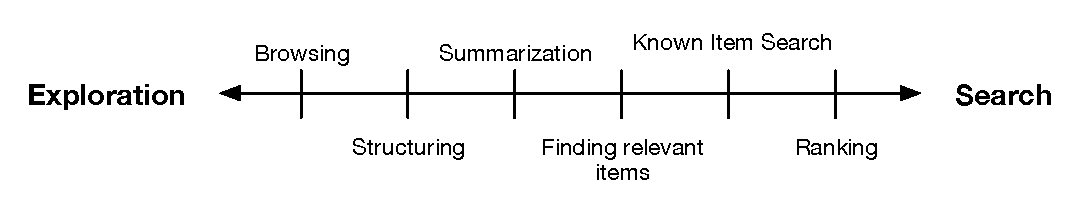
\includegraphics[width=\textwidth]{figures/exploration_search_axis.eps}
    \caption{Exploration-search axis of multimedia analytics~\cite{Zahalka:2014Towards}.}
    \label{figure:exploration-search-axis}
\end{figure}

For analytics on a multimedia collection Zahálka and Worring \cite{Zahalka:2014Towards} propose the formal model of an \emph{exploration-search axis}, which is depicted in \cref{figure:exploration-search-axis}. The model is used to characterise the different types of tasks carried out by the user. The axis specifies two ends of a spectrum, with \emph{exploration} marking one end -- if the user knows nothing about the data collection -- and \emph{search} marking the other end -- if the user knows exactly which specific items of a collection they are interested in. During a multimedia analytics task a user's activities often oscillate between the two ends of the spectrum until the desired knowledge has been generated. Unsurprisingly, all the depicted activities come with distinct requirements on data transformation and processing.

\subsection{Multimedia Retrieval}

Traditionally, multimedia retrieval has been regarded as a special niche within the  multimedia analysis domain. It constitutes a dedicated field of research that deals with searching and finding items of interest within large bodies of (multi)-media data, based on information that may not necessarily be available in a structured manner, such as, motives depicted in an image. Even though search and retrieval may sound like the main function offered by a database, it is a very different task for multimedia than it is for structured data~\cite{Blanken:2007multimedia}. On the one hand, given the structure of, e.g., a relational database and languages like \acrshort{sql}, a user can specify exactly what elements from the database should be selected using predicates that lead to a binary decision whether items in a collection match or not. For example, when considering a product database that contains price information for individual items on sale, it is easy to formulate a query that selects all items above a specific price threshold.

Retrieving multimedia data, on the other hand, comes with indirections due to the unstructured nature of the content, the feature representations used as a proxy for it and the \emph{semantic gap} \cite{Blanken:2007multimedia, Rossetto:2018Multi} associated with them. A very popular model to work with feature representation in multimedia retrieval involves calculation of (dis-)similarity scores from the features and sorting and ranking of items based on this score. This is commonly referred to as the \emph{vector space model} of multimedia retrieval and similarity search \cite{Zezula:2006Similarity}. It is inherently non-binary in nature, i.e., an item matches a query to some degree and may be among the results even though the score indicates that it is a bad match. Over the years, many different combinations of features and ranking models have been proposed to facilitate content-based retrieval of different media types, such as images, audio, or video \cite{Hu:2011Survey,Dharani:2013Survey,Murthy:2018Content} as have been different types of query formulation, that complement traditional, text-based input. These models include methods such as \emph{Query-by-Example} \cite{Kelly:1995Query}, \emph{Query-by-Sketch} \cite{Sciascio:1999Content}, \emph{Query-by-Humming} \cite{Ghias:1995query} or \emph{Query-by-Sculpting}~\cite{Boerlin:20203d}.

It is worth noting, that when considering concrete, ``real-world'' multimedia retrieval system implementations today, the lines between traditional multimedia retrieval and multimedia analytics quickly start to blur. This is because traditional multimedia retrieval operates under the assumption that a specific retrieval model produces the correct result in the top ranks (e.g. the top 5) and that an item can thus be retrieved by a single query. In practice, this is often not the case due to limitations of the model itself, imprecisions in the query or simply because an information need may be very general rather than specific. Therefore, finding an item of interest often requires multiple queries and other types of interaction with the data collection. This is sometimes referred to interactive multimedia retrieval and it usually includes a user in the loop.

Therefore, in addition to the extraction of appropriate features and the conception of effective ranking algorithms, interactive multimedia retrieval systems also concern themselves with aspects such as query (re-)formulation and refinement, results presentation and efficient exploration~\cite{Lokovc:2019Interactive}. Moreover, such systems do not simply operate on feature representations anymore but combine similarity and Boolean search ~\cite{Rossetto:2020Interactive}. Consequently, one could argue that interactive multimedia retrieval systems perform a specific type of multimedia analytics task, which is that of finding unknown items that satisfy a specific information need. This makes all the arguments made about data processing and data management requirements for multimedia analytics applicable to interactive multimedia retrieval as well.

\subsection{Multimedia Data Management}

As (multi-)media collections become large enough for the relevant units of information to no longer fit into main memory (\acrshort{ram}), multimedia retrieval and analytics quickly become issues of scalable data management~\cite{Jonsson:2016Ten,Pouyanfar:2018}. Therefore, it is no longer just a question of effective feature engineering and ranking but also of strategies to store and index the original data as well as derived descriptors in a way that allows for efficient and effective processing in the face of interactive users, changing query workloads and changing data \cite{Smeulders:2000Content}. This data management aspect brings about many challenges that do, however, bear some similarity with problems that have already been addressed in database research.

However, as of today, state of the art in multimedia analytics \emph{``[...] has up to now [...] not explicitly considered the issue of data management, despite aiming for large-scale analytics.''} \cite{Jonsson:2016Ten} (p. 296), a statement that can also be made about multimedia retrieval In contrast, the database research community has identified the support for unstructured and multimedia data as well as the integration of information retrieval and database functionality as important research directions in both the \emph{Lowell} and the \emph{Claremont} reports on the state of database research in 2005 and 2008, respectively \cite{Abiteboul:2005Lowell,Agrawal:2008Claremont}. Despite these initiatives, however, the two fields have remained largely disjointed areas of research until today, with only a few isolated contributions that straddle the two.

\section{Research Gap and Objective}
\label{section:research_gap}

Despite some theoretical work towards multimedia data management \cite{Marcus:1996Foundations,Adjeroh:1997Multimedia}, the conception of concrete multimedia database systems~\cite{Giangreco:2016Adam,Yang:2020Pase,Wang:2021Milvus} as well as multimedia retrieval systems that refactor data management into distinct components~\cite{Carey:1995Towards,Rossetto:2016Vitrivr,Gasser:2019Multimodal}, there is still a gaping disconnect between multimedia retrieval, analytics and database research. While~\cite{Giangreco:2018Database} proposes important contributions towards a unified data-, query- and execution-model required for effective search in multimedia collections, scalability aspects and the need for near real-time query performance, especially in the face of changing data, are not systematically considered. Contrarily, the proposed models -- despite being seminal for data management in multimedia retrieval applications -- postulate assumptions, that have considerable impact on the practical applicability of systems implementing them.

The starting point for the research described in this thesis is therefore the current state-of-the-art for data management in multimedia retrieval and analytics, as briefly touched upon in the previous sections. Starting from and inspired by the models and solutions proposed in \cite{Giangreco:2016Adam,Giangreco:2018Database} and motivated by the ``Ten Research Questions for Scalable Multimedia Analytics''~\cite{Jonsson:2016Ten}, this thesis challenges three basic assumptions currently employed and operated upon in multimedia data management and explores the ramifications of doing so, with the higher-level goal of bridging certain gaps between research conducted in multimedia retrieval, analysis and analytics on the one hand, and classical data management and databases on the other. These assumptions are:

\begin{description}
    \item[Assumption 1: Nearest Neighbour Search] The metric space model employed in multimedia retrieval \cite{Zezula:2006Similarity} relies on a notion of similarity search that is usually expressed as finding the $k$ nearest neighbouring feature vectors $f_{i \in \left[1,k\right]} \in \symfeatures$ to a query vector $q \in \symreal^d$ in a collection $\symfeatures \subset \symreal^d$ given a certain distance function. A common strategy to accommodate this type of search is to add this operation as a new query primitive in addition to whatever an existing data model might already bring \cite{Guliato:2009PostgreSQL,Giangreco:2016Adam,Yang:2020Pase}, without systematically considering the interplay between this primitive and other database operations.

    \item[Assumption 2: Staticity of Data Collections] Multimedia retrieval systems today often make a distinction between an \emph{offline} phase, during which media items are analysed, features are generated, and derived data is ingested into a data management system, and an \emph{online} phase, during which queries take place. Usually, no changes to the data collection are allowed during the online phase. This model is, for example, advertised by \cite{Flickner:1995Query,Kiranyaz:2003Muvis,Giangreco:2018Database,Rossetto:2018Multi} and to the best of our knowledge, most existing multimedia retrieval and analytics systems implement this either explicitly or implicitly, with a few exceptions, such as the system presented in \cite{Wang:2021Milvus}.

    \item[Assumption 3: User Driven Query Execution] Database systems usually evaluate and select the execution plan for an incoming query during a step that is referred to as \emph{query planning}. The underlying assumption is that the database has all the information required to determine the most effective execution path in terms of cost parameters, such as required \acrshort{io}, \acrshort{cpu}, and memory usage. In contrast, this is often not the case for multimedia retrieval systems and instead, it falls to the user to make decisions as to how a query should be executed, e.g., in terms of indexes that should be employed.
\end{description}

On the issue of Assumption 1, one can say that while the described model may be very concise and simple to implement, it merely allows for the ranking of results and is therefore only able to accommodate the search-end of the \emph{exploration-search axis}, assuming that features are, in fact, real-valued vectors. However, the model cannot be generalised to other operations that involve distance calculation and becomes too limited for tasks such as browsing, structuring and summarization, thus delegating the required data processing to upper-tier system components. Referring to \cite{Jonsson:2016Ten}, it would however be desirable to offer such primitives at a database level. Furthermore, the metric space model with its \acrfull{nns} paradigm may be too limited for certain use-cases and a broader range of operations therefore be preferable.

It is also worth noting, that Assumption 2 and 3 both go against well established design principles usually found in modern database systems~\cite{Petrov:2019Database,Amsaleg:2014Database}. While it may be convenient from a perspective of system design, to assume a data collection to be static -- because we do not have to deal with transaction isolation -- this is almost never the case and such a mode of operation is utterly limiting when considering data that is subject to incremental change, e.g., when performing online analytics or when working with applications that offer \acrshort{crud} support. A similar argument can be made for the manual selection of query execution paths. Even though it may be simplifying the process of query planning, such a design decision (falsely) assumes, that a user is always a technical expert and that all the potential query workloads are known in advance. Consequently, it limits the optimisation options available to the system. 

On a more general point, it cannot be assumed that all the query workloads a multimedia database management system must handle can be anticipated at build time, especially if a session involves a user in the loop. This was emphasised by Smeulders at al. in 2000 already, who stated that \emph{``the interacting user brings about many new challenges for the response time of the system. Content-based image retrieval is only scalable to large data sets when the database is able to anticipate what interactive queries will be made. A frequent assumption is that the image set, the features, and the similarity function are known in advance. In a truly interactive session, the assumptions are no longer valid. A change from static to dynamic indexing is required.''} \cite{Smeulders:2000Content} (p. 1369). This statement is still of high, practical relevance and summarises what we have expressed in the three assumptions. It can thus be regarded as yet another argument to consider multimedia data management as an important and interesting research challenge.

%\subsection{Research Questions}

%Challenging the aforementioned assumptions raises very specific questions that fundamentaly impact the design of a \emph{multimedia data management system}. These questions are briefly summarized in \cref{table:research_questions}.

%\begin{table}[h!]
%    \centering
%    \caption{List of research questions (RQ) resulting from challenging assumptions(AS) one, two and three.}
%   \begin{tabular}{|c|p{10cm}|c|c|} 
%    \hline
%    \textbf{RQ} & \textbf{Question} & \textbf{Assumption} & \textbf{Domain} \\ [0.5ex] 
%    \hline\hline
%     1 & Which commonly used, secondary index structures for NNS (e.g., VA \cite{Weber:1998Va}, LSH \cite{Indyk1998:Approximate}, PQ \cite{Jegou:2010Product} based indexes) can cope with changes to data and to what extent? & AS 1 &\\ 
%    2 & Can we estimate and quantify deterioration of retrieval quality of index structures from RQ1 as changes are being made to the underlying data collections? & AS 1 & \\ 
%    3 & How can we handle index structures from RQ1 for which to expect deterioration during query planning and execution? & AS 1 & \\
%    4 & Can we devise a model that (temporarily) compensates deterioration of retrieval quality of index structures? & AS 1 & \\
%    5 & How can user knowledge about the the retrieval task at hand be factored into query planning without forcing the user the make explicit choices about how a query should be executed? & AS 1 \& 3 & \\
%    6 & How would a cost model that factors in desired retrieval accuracy look like and can it be applied during query planning? & AS 3 & \\ 
%    7 & Assuming the cost model in RQ6 exists, at what levels of the system can it be applied (globally, per query, context)? & AS 3 & \\ 
%    8 & Is there a measurable impact (e.g., on query execution time vs. accuracy) of having such a cost model? & AS 3 & \\ 
%    9 & Can we generalize the model for similarity search (i.e., the vector space model) and what is the consequence of doing so? & AS 2 & \\ 
%    10 & Do the existing applications and use-cases justify a generalization? & AS 2 & \\ 
%    \hline
%   \end{tabular}
%   \label{table:research_questions}
%\end{table}

%RQ1 to RQ5 address the issue of index structures for NNS, which are mostly unable to cope with data that is subject to change, since their correctness deteriorates as data is modified. The focus of these questions are whether deterioration can be quantified and how it can be handled by a system. We argue, that both is necessary for practical application in dynamic data management.

%RQ6 to RQ8 explore the possibility of a cost model, that takes accuracy of the produced results into account. Since most techniques for fast NNS rely on approximation, inaccuracy is an inherent factor for such operations. Assuming such a model exists, it can be used by a user or system administrator to make explicit choices between either accuracy or execution peformance. In addition, such a cost model can be put to use when deciding what indexes to use in face of deteriorated retrieval quality due to changing data.

%And finally, RQ9 and RQ10 address the issue of a more generalized model for similarity search and the impact of such a model on all the different system components. Most importantly, however, they explore and justify the need for such a model, which is not self-evident, based on concrete use-cases and applications.

\section{Contribution and Outline}
\label{section:contributions}

In this thesis we address the research gaps identified in \cref{section:research_gap} and thereby try to bridge the disparity between the fields of databases and multimedia retrieval systems. The contribution of this thesis can be summarized as follows:

\begin{itemize}
    \item We propose a \emph{generalised model for proximity based search} as an extension to the relational data model and explore the implications of such a model on aspects, such as, optimisation of query execution time and query planning.
    \item We examine the impact of challenging the \emph{data staticity assumption} on index structures commonly used for similarity search and describe an \emph{high-dimensional index maintenance} model by which a multimedia database system can cope with and make sense of changing index structures.
    \item We propose a \emph{cost model that factors in quality} of generated results in addition to common performance metrics, and, based on that model, derive mechanisms for the user to express their preference for either accuracy or speed at different levels of the system.
    \item We introduce the multimedia database \emph{Cottontail DB}~\cite{Gasser:2020Cottontail} that implements the aforementioned models and present an evaluation thereof.
\end{itemize}

This thesis is presented in four parts, each of which consists of several chapters that incrementally build on one another.

\begin{description}
    \item[Part I] provides an introduction and problem statement (\cref{chapter:introduction}) and describes motivating use cases and the requirements they bring (\cref{chapter:applications}).
    \item[Part II] gives a brief summary of the theoretical foundation and state of the art in database (\cref{chapter:theory_databases}) and multimedia analysis and retrieval (\cref{chapter:theory_multimedia_analysis_and_retrieval}) research and tries to combine the two aspects on a systems level in a brief survey of multimedia database systems (\Cref{chapter:theory_multimedia_database}). In addition to establishing a common foundation and framework for the remainder of this thesis, we also use this part to survey related work.
    \item[Part III] formalises the theoretical models that make up the contributions (\cref{chapter:system_model}) and introduces and describes our reference implementation Cottontail DB (\cref{chapter:cottontaildb}).
    \item[Part IV] presents and discusses the evaluation of the contributions (\cref{chapter:evaluation}) and provides a conclusion (\cref{chapter:conclusion}).
\end{description}